\documentclass[titlepage]{jarticle}
\usepackage{h31ec-exp}
\usepackage[dvipdfmx]{graphicx}
\usepackage[yen]{okuverb}
\usepackage{here}

\title{半導体素子の静特性の測定}
\grade{3年41番}%
\author{鷲尾 優作}
\team{}
\date{令和3年6月14日,6月21日,6月28日}
\expdate{令和3年6月28日}
\coauthor{
  39番 & 宮崎 来\\
  42番 & 渡辺 あかり\\
  %34番 & 西脇 光
}

\begin{document}
\maketitle

%目次の出力
\tableofcontents
\newpage

\section{実験A ダイオードとツェナーダイオードの静特性}
\subsection{目的}
\begin{itemize}
    \item pn接合半導体素子(ダイオード)の順方向,逆方向の電圧-電流特性を測定する.
    \item 逆方向の電圧を増加させた時に,ある電圧になると電流が急増する降伏特性を利用したツェナダイオードの電圧-電流特性を測定する.
    \item 交流入力に対する半波整流特性を観測することにより,ダイオードの整流特性について学習する.
\end{itemize}
\subsection{使用器具}
\begin{enumerate}
    \item ダイオード静特性評価回路 EC-01
    \item 直流安定化電源装置 TAKASAGO GPO25-5 帳1 番号195 分類B21
    \item 交流電源装置 KENWOOD AG-203 EC-02
    \item デジタルマルチメータ SANWA CD770 EC-34
    \item オシロスコープ GWINSTEK GDS-1022 No.6
\end{enumerate}
\subsection{ダイオードの静特性}

\subsubsection{順方向の特性}
整流用ダイオード順方向に印加する電圧を変化させ,電圧電流特性を測定する.
ダイオードの端子間電圧はダイオードの定格電流を考え,0-5[V]を超えないよう測定した.
精密な測定を図るため,ダイオードと直列に接続した抵抗器の両端電圧を測定し,キルヒホッフの法則を利用し
間接的にダイオードの両端電圧を測定する方法を用いた,

以下図\ref{fig:ダイオードの順方向静特性測定回路}に測定対象の回路図を示す.
\begin{figure}[H]
    \begin{center}
        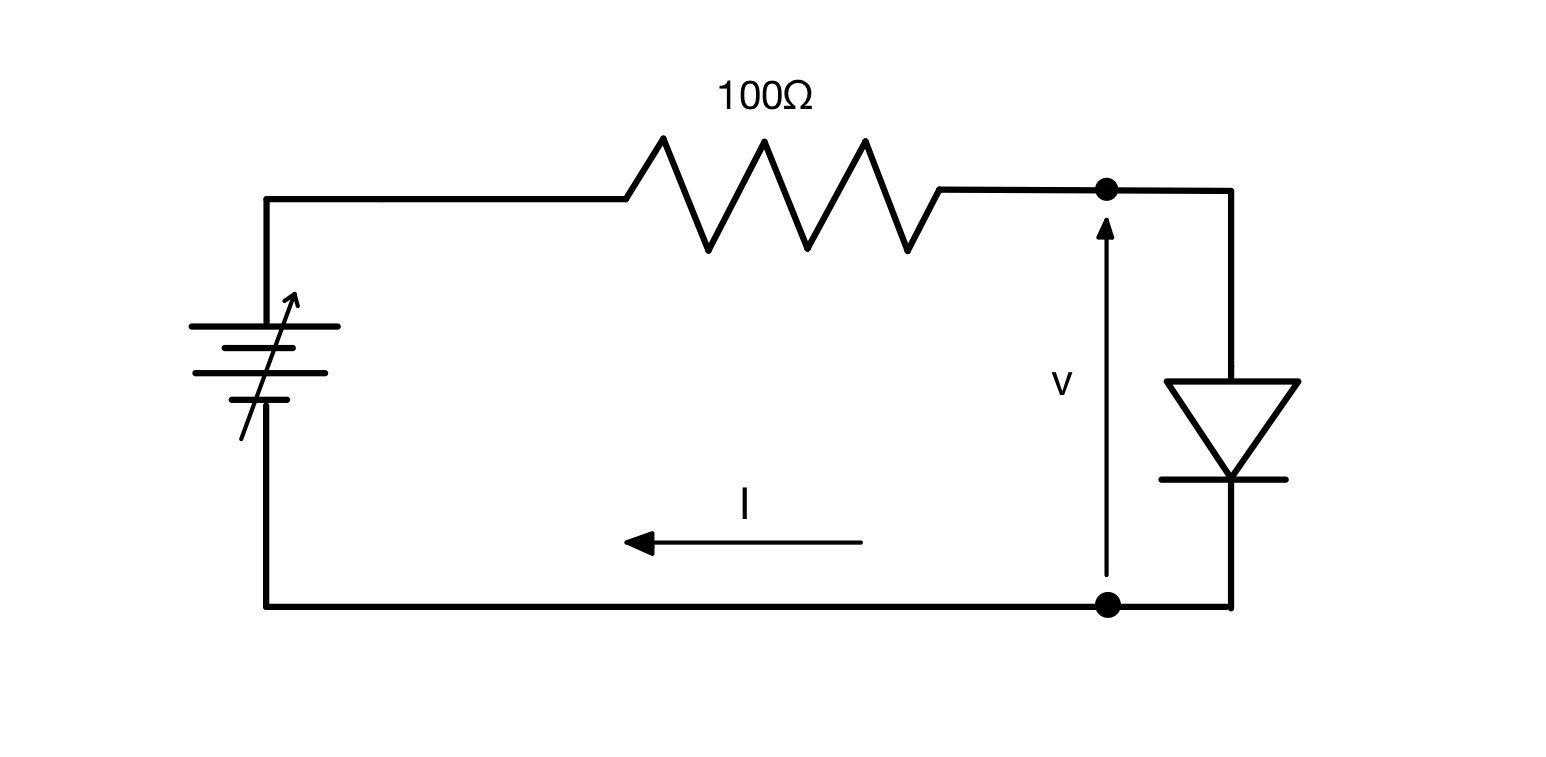
\includegraphics[width=10cm]{image/dt.jpg}
        \caption{ダイオードの順方向静特性測定回路}
        \label{fig:ダイオードの順方向静特性測定回路}
    \end{center}
\end{figure}

表\ref{ダイオード順方向バイアスにおける電圧電流特性測定結果}に測定によって得られた結果を示す.
また,以下図\ref{fig:ダイオード順方向バイアスにおける電圧電流特性(グラフ)}にグラフを示す.

測定結果は変化の大きい部分を重点的に測定しており,不均一なものしている.
結果からはダイオード両端電圧が0.5[V]を超えたところで徐々に電流が流れ出し,0.8[V]にかけて急激に増加していく様子がわかる.
これは,順方向電圧の印加によって内部電界が打ち消され,空乏層が減少することで通過可能な電流が増加したためである.
\begin{table}[htbp]
    \caption{ダイオード順方向バイアスにおける電圧電流特性測定結果}
    \begin{center}
        \begin{tabular}{r|r|r|r}
            \hline\hline
            \multicolumn{1}{l|}{抵抗にかかる電圧[V]} & \multicolumn{1}{l|}{主電源E[V]} & \multicolumn{1}{l|}{ダイオード両端電圧「V]} & \multicolumn{1}{l}{電流[mA]} \\ \hline
            4.960                                    & 5.730                           & 0.770                                       & 49.6                         \\ \hline
            3.030                                    & 3.773                           & 0.743                                       & 30.3                         \\ \hline
            1.508                                    & 2.220                           & 0.712                                       & 15.08                        \\ \hline
            0.996                                    & 1.691                           & 0.695                                       & 9.96                         \\ \hline
            0.511                                    & 1.177                           & 0.666                                       & 5.11                         \\ \hline
            0.252                                    & 0.887                           & 0.635                                       & 2.52                         \\ \hline
            0.095                                    & 0.688                           & 0.593                                       & 0.95                         \\ \hline
            0.051                                    & 0.617                           & 0.566                                       & 0.51                         \\ \hline
            0.025                                    & 0.559                           & 0.534                                       & 0.25                         \\ \hline
            0.013                                    & 0.521                           & 0.508                                       & 0.13                         \\ \hline
            0.005                                    & 0.478                           & 0.473                                       & 0.05                         \\ \hline
            0.000                                    & -0.020                          & -0.020                                      & 0                            \\ \hline
        \end{tabular}
    \end{center}
    \label{ダイオード順方向バイアスにおける電圧電流特性測定結果}
\end{table}


\begin{figure}[H]
    \begin{center}
        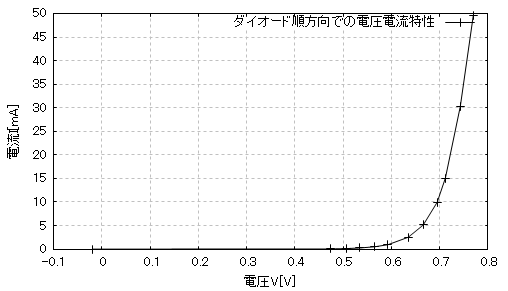
\includegraphics[width=10cm]{graph/1.png}
        \caption{ダイオード順方向バイアスにおける電圧電流特性(グラフ)}
        \label{fig:ダイオード順方向バイアスにおける電圧電流特性(グラフ)}
    \end{center}
\end{figure}

\subsubsection{逆方向の特性}
同様に逆方向電圧を印加し,電圧電流特性を測定する.

設定電圧,測定方法については前項と同じ方法を用いている.

以下図\ref{fig:ダイオードの逆方向静特性測定回路}に測定対象の回路図を示す.
\begin{figure}[H]
    \begin{center}
        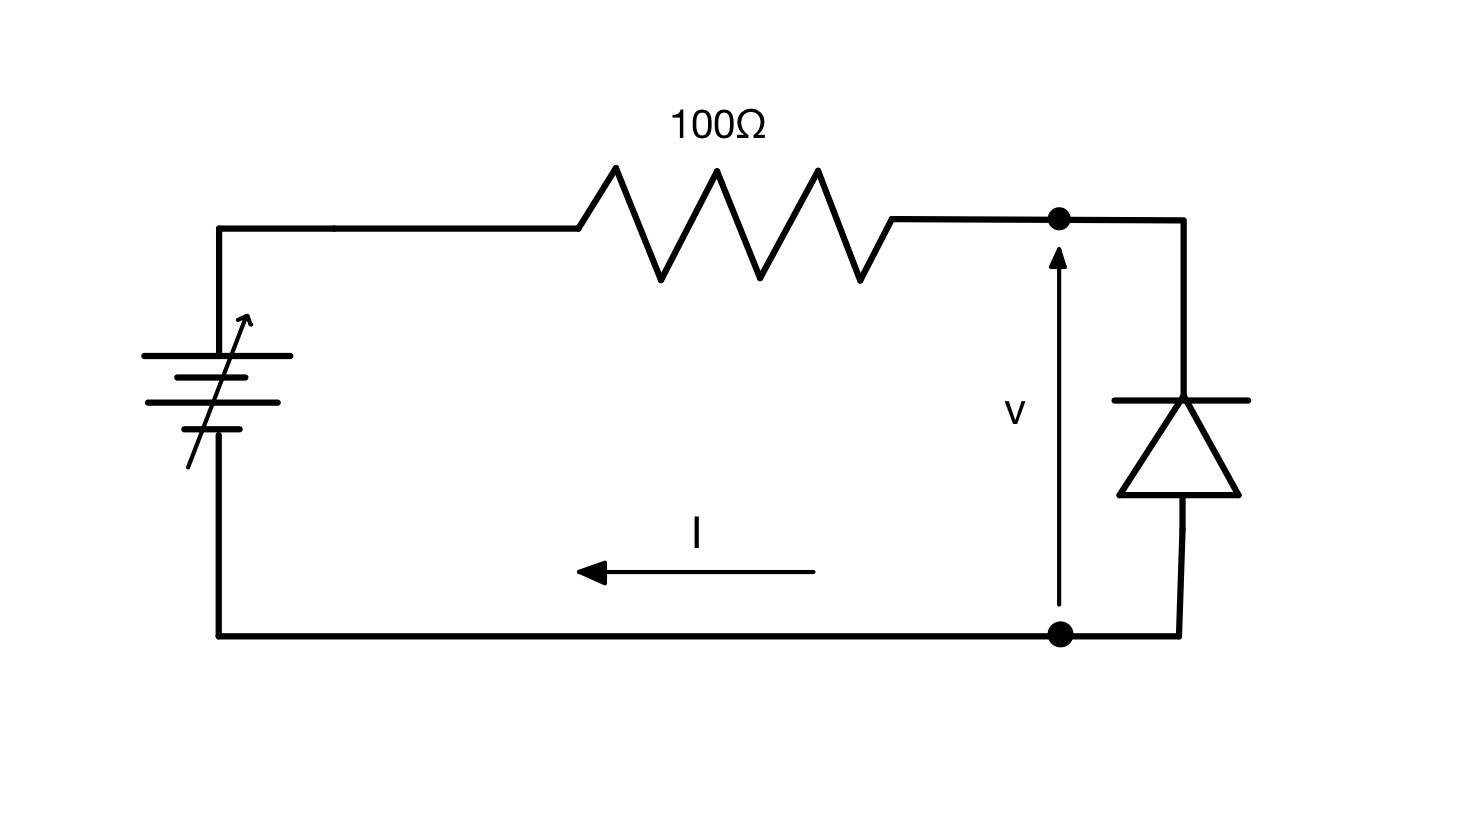
\includegraphics[width=10cm]{image/db.jpg}
        \caption{ダイオードの逆方向静特性測定回路}
        \label{fig:ダイオードの逆方向静特性測定回路}
    \end{center}
\end{figure}

以下表\ref{ダイオード逆方向バイアスにおける電圧電流特性測定結果}に得られた測定値を示す.

\begin{table}[htbp]
    \caption{ダイオード逆方向バイアスにおける電圧電流特性測定結果}
    \begin{center}
        \begin{tabular}{r|r|r|r}
            \hline\hline
            \multicolumn{1}{l|}{抵抗にかかる電圧[V]} & \multicolumn{1}{l|}{主電源E[V]} & \multicolumn{1}{l|}{ダイオードに印加する電圧「V]} & \multicolumn{1}{l}{電流[mA]} \\ \hline
            0.000                                    & -4.940                          & -4.940                                            & 0                            \\ \hline
            -0.001                                   & -3.039                          & -3.038                                            & -0.01                        \\ \hline
            0.000                                    & -1.055                          & -1.055                                            & 0                            \\ \hline
            0.000                                    & -0.493                          & -0.493                                            & 0                            \\ \hline
            0.000                                    & -0.098                          & -0.098                                            & 0                            \\ \hline
        \end{tabular}
    \end{center}
    \label{ダイオード逆方向バイアスにおける電圧電流特性測定結果}
\end{table}

図\ref{fig:ダイオード逆方向バイアスにおける電圧電流特性(グラフ)}にグラフを示す.
逆バイアス下においては電圧の変化に対して電流はほとんど流れない状態で変わらないことがわかる.
印加した電圧が内部電界を拡張する方向にはたらき,空乏層が拡大し絶縁性が増すためである.
ダイオードの持つ整流作用が正常に働いていると考えられる.

\begin{figure}[H]
    \begin{center}
        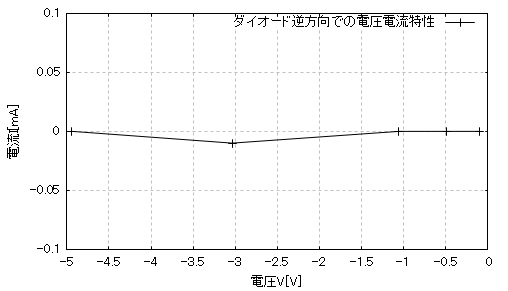
\includegraphics[width=10cm]{graph/2.png}
        \caption{ダイオード逆方向バイアスにおける電圧電流特性(グラフ)}
        \label{fig:ダイオード逆方向バイアスにおける電圧電流特性(グラフ)}
    \end{center}
\end{figure}

\subsection{ツェナーダイオードの静特性}
ツェナーダイオード順方向に印加する電圧を変化させ,電圧電流特性を測定する.
ダイオードの端子間電圧は先ほどの実験と同様にダイオードの定格電流を考え,0-5[V]を超えないよう測定した.
精密な測定を図るため,ダイオードと直列に接続した抵抗器の両端電圧を測定し,キルヒホッフの法則を利用し
間接的にツェナーダイオードの両端電圧を測定する方法を用いた,

以下図\ref{fig:ツェナーダイオードの順方向静特性測定回路}に測定対象の回路図を示す.
\subsubsection{順方向の特性}
\begin{figure}[H]
    \begin{center}
        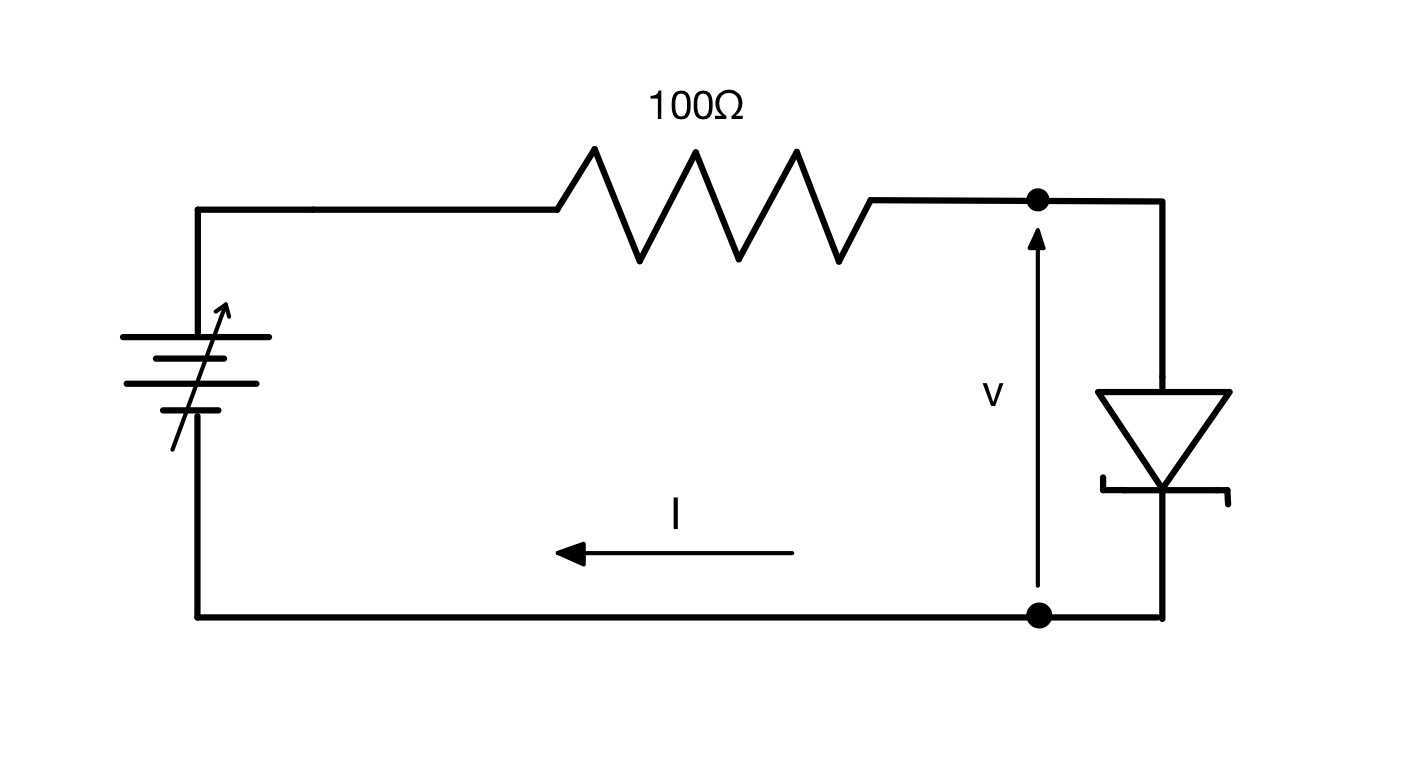
\includegraphics[width=10cm]{image/tt.jpg}
        \caption{ツェナーダイオードの順方向静特性測定回路}
        \label{fig:ツェナーダイオードの順方向静特性測定回路}
    \end{center}
\end{figure}

以下表\ref{ツェナーダイオード順方向バイアスにおける電圧電流特性測定結果}に測定結果を示す.

\begin{table}[htbp]
    \caption{ツェナーダイオード順方向バイアスにおける電圧電流特性測定結果}
    \begin{center}
        \begin{tabular}{r|r|r|r}
            \hline\hline
            \multicolumn{1}{l|}{抵抗にかかる電圧[V]} & \multicolumn{1}{l|}{主電源E[V]} & \multicolumn{1}{l|}{ダイオードに印加する電圧「V]} & \multicolumn{1}{l}{電流[mA]} \\ \hline
            4.990                                    & 5.760                           & 0.770                                             & 49.9                         \\ \hline
            2.494                                    & 3.251                           & 0.757                                             & 24.94                        \\ \hline
            1.502                                    & 2.247                           & 0.745                                             & 15.02                        \\ \hline
            0.522                                    & 1.240                           & 0.718                                             & 5.22                         \\ \hline
            0.246                                    & 0.945                           & 0.699                                             & 2.46                         \\ \hline
            0.199                                    & 0.892                           & 0.693                                             & 1.99                         \\ \hline
            0.146                                    & 0.831                           & 0.685                                             & 1.46                         \\ \hline
            0.098                                    & 0.774                           & 0.676                                             & 0.98                         \\ \hline
            0.049                                    & 0.707                           & 0.658                                             & 0.49                         \\ \hline
            0.024                                    & 0.664                           & 0.640                                             & 0.24                         \\ \hline
            0.006                                    & 0.607                           & 0.601                                             & 0.06                         \\ \hline
            0.002                                    & 0.574                           & 0.572                                             & 0.02                         \\ \hline
            0.000                                    & 0.503                           & 0.503                                             & 0                            \\ \hline
        \end{tabular}
    \end{center}
    \label{ツェナーダイオード順方向バイアスにおける電圧電流特性測定結果}
\end{table}

図\ref{fig:ツェナーダイオード順方向バイアスにおける電圧電流特性(グラフ)}にグラフ化したものを示す.
グラフの外形,特徴は整流用ダイオードと酷似しており,ダイオード同様に0.5[V]から0.8[V]にかけて急激に電流が変化している.
ツェナーダイオードでも順方向特性は一般的なダイオードと同様の特性を示すことがわかる.

\begin{figure}[H]
    \begin{center}
        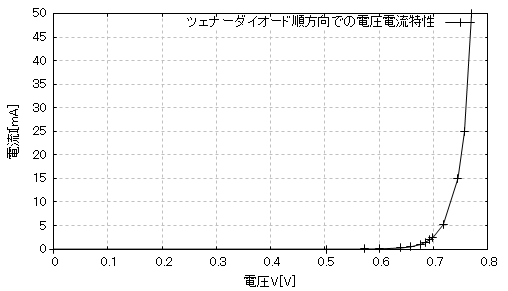
\includegraphics[width=10cm]{graph/3.png}
        \caption{ツェナーダイオード順方向バイアスにおける電圧電流特性(グラフ)}
        \label{fig:ツェナーダイオード順方向バイアスにおける電圧電流特性(グラフ)}
    \end{center}
\end{figure}

\subsubsection{逆方向の特性}
同様に逆方向電圧を印加し,電圧電流特性を測定する.
測定方法については前項と同じ方法を用いる.

以下図\ref{fig:ツェナーダイオードの逆方向静特性測定回路}に測定対象の回路図を示す.
\begin{figure}[H]
    \begin{center}
        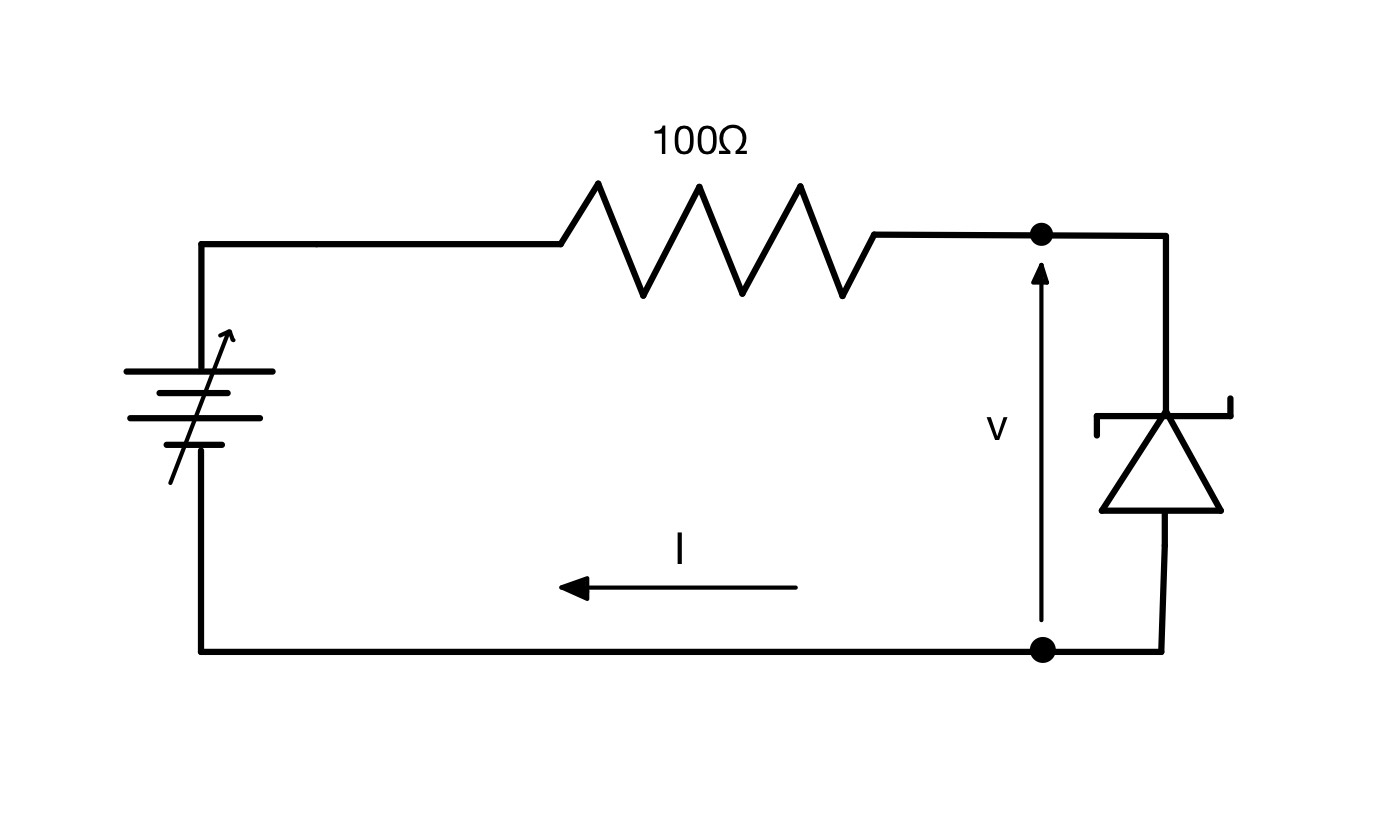
\includegraphics[width=10cm]{image/tb.jpg}
        \caption{ツェナーダイオードの逆方向静特性測定回路}
        \label{fig:ツェナーダイオードの逆方向静特性測定回路}
    \end{center}
\end{figure}

表\ref{ツェナーダイオード逆方向バイアスにおける電圧電流特性測定結果}に測定によって得られた結果を示す.
\begin{table}[htbp]
    \caption{ツェナーダイオード逆方向バイアスにおける電圧電流特性測定結果}
    \begin{center}
        \begin{tabular}{r|r|r|r}
            \hline\hline
            \multicolumn{1}{l|}{抵抗にかかる電圧[V]} & \multicolumn{1}{l|}{主電源E[V]} & \multicolumn{1}{l|}{ダイオードに印加する電圧「V]} & \multicolumn{1}{l}{電流[mA]} \\ \hline
            -5.000                                   & -11.30                          & -6.300                                            & -50                          \\ \hline
            -2.497                                   & -8.810                          & -6.313                                            & -24.97                       \\ \hline
            -1.013                                   & -7.280                          & -6.267                                            & -10.13                       \\ \hline
            -0.490                                   & -6.740                          & -6.25                                             & -4.9                         \\ \hline
            -0.206                                   & -6.430                          & -6.224                                            & -2.06                        \\ \hline
            -0.150                                   & -6.360                          & -6.21                                             & -1.5                         \\ \hline
            -0.068                                   & -6.250                          & -6.182                                            & -0.68                        \\ \hline
            -0.039                                   & -6.160                          & -6.121                                            & -0.39                        \\ \hline
            -0.025                                   & -6.080                          & -6.055                                            & -0.25                        \\ \hline
            -0.019                                   & -6.040                          & -6.021                                            & -0.19                        \\ \hline
            -0.014                                   & -5.980                          & -5.966                                            & -0.14                        \\ \hline
            -0.010                                   & -5.910                          & -5.900                                            & -0.1                         \\ \hline
            -0.005                                   & -5.740                          & -5.735                                            & -0.05                        \\ \hline
            0.000                                    & -5.730                          & -5.73                                             & 0                            \\ \hline
            0.001                                    & -2.012                          & -2.013                                            & 0.01                         \\ \hline
            0.000                                    & -1.061                          & -1.061                                            & 0                            \\ \hline
            0.000                                    & -0.488                          & -0.488                                            & 0                            \\ \hline
        \end{tabular}
    \end{center}
    \label{ツェナーダイオード逆方向バイアスにおける電圧電流特性測定結果}
\end{table}

図\ref{fig:ツェナーダイオード逆方向バイアスにおける電圧電流特性(グラフ)}にグラフを示す.

6[V]を下回ったところで急激に電流が流れだすツェナーダイオード特有の特性が見られる.
ツェナーダイオードは逆バイアス下一定の電圧を超えたときこのような特性が得られるよう作られており
回路内で電圧,電流を安定させる用途で多用される.
このツェナーダイオードはおよそ6[V]で安定するよう設計されていると考えられる.

\begin{figure}[H]
    \begin{center}
        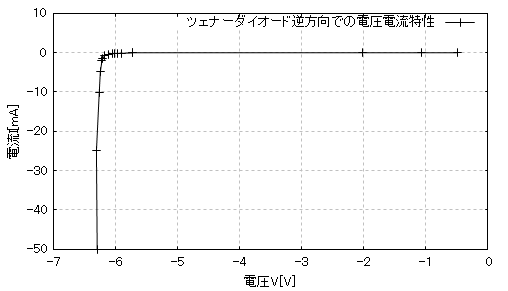
\includegraphics[width=10cm]{graph/4.png}
        \caption{ツェナーダイオード逆方向バイアスにおける電圧電流特性(グラフ)}
        \label{fig:ツェナーダイオード逆方向バイアスにおける電圧電流特性(グラフ)}
    \end{center}
\end{figure}

\subsection{ダイオードの半波整流特性}
周波数100[Hz],振幅5[V]の正弦波をLFOを用いて回路に入力し.

オシロスコープch1でLFOの出力を監視し,ch2でダイオードの両端電圧を監視する.
この時の波形の様子を観察,報告する.

以下図\ref{fig:半波整流回路}に測定対象の半波整流回路を示す.
\begin{figure}[H]
    \begin{center}
        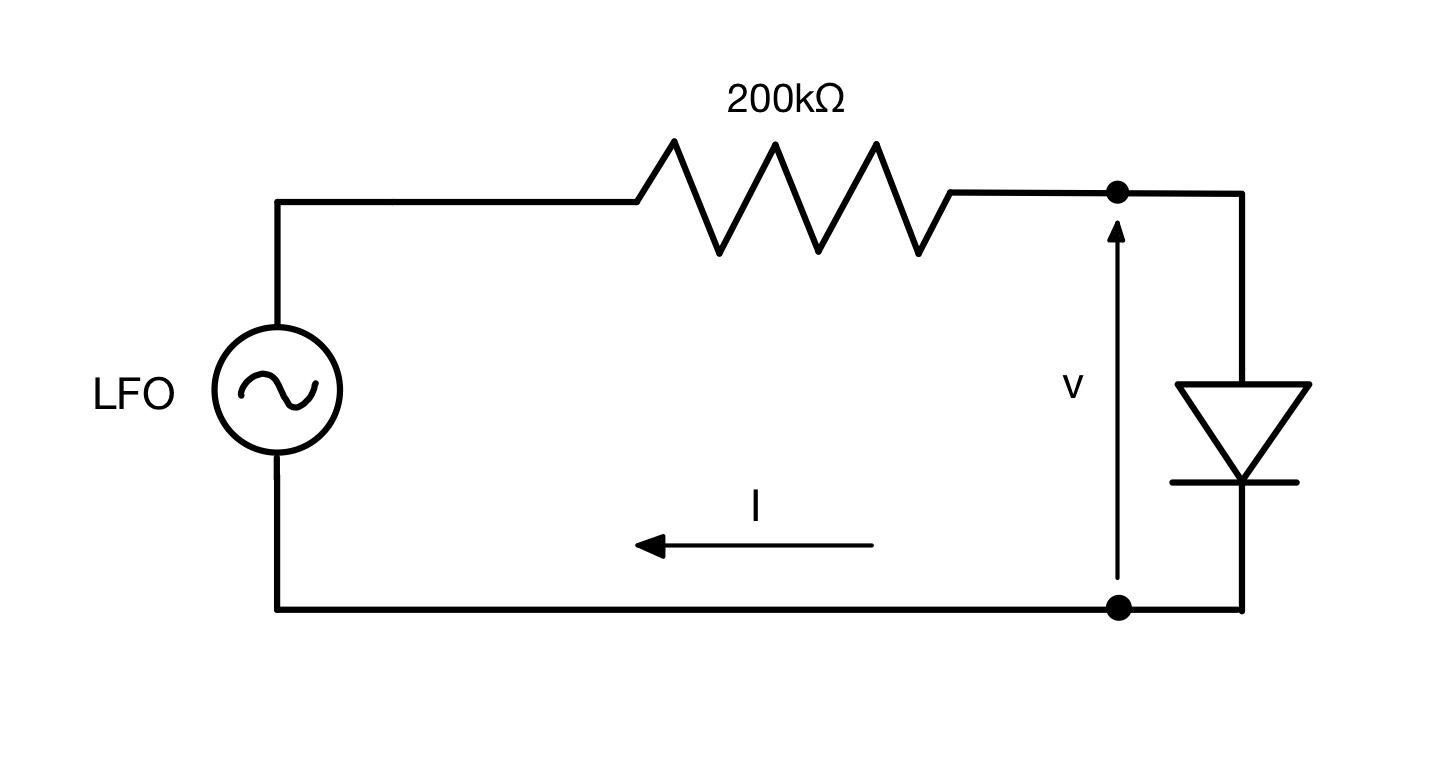
\includegraphics[width=10cm]{image/lfo.jpg}
        \caption{半波整流回路}
        \label{fig:半波整流回路}
    \end{center}
\end{figure}

測定中のオシロスコープの波形を示す.
\begin{figure}[H]
    \begin{center}
        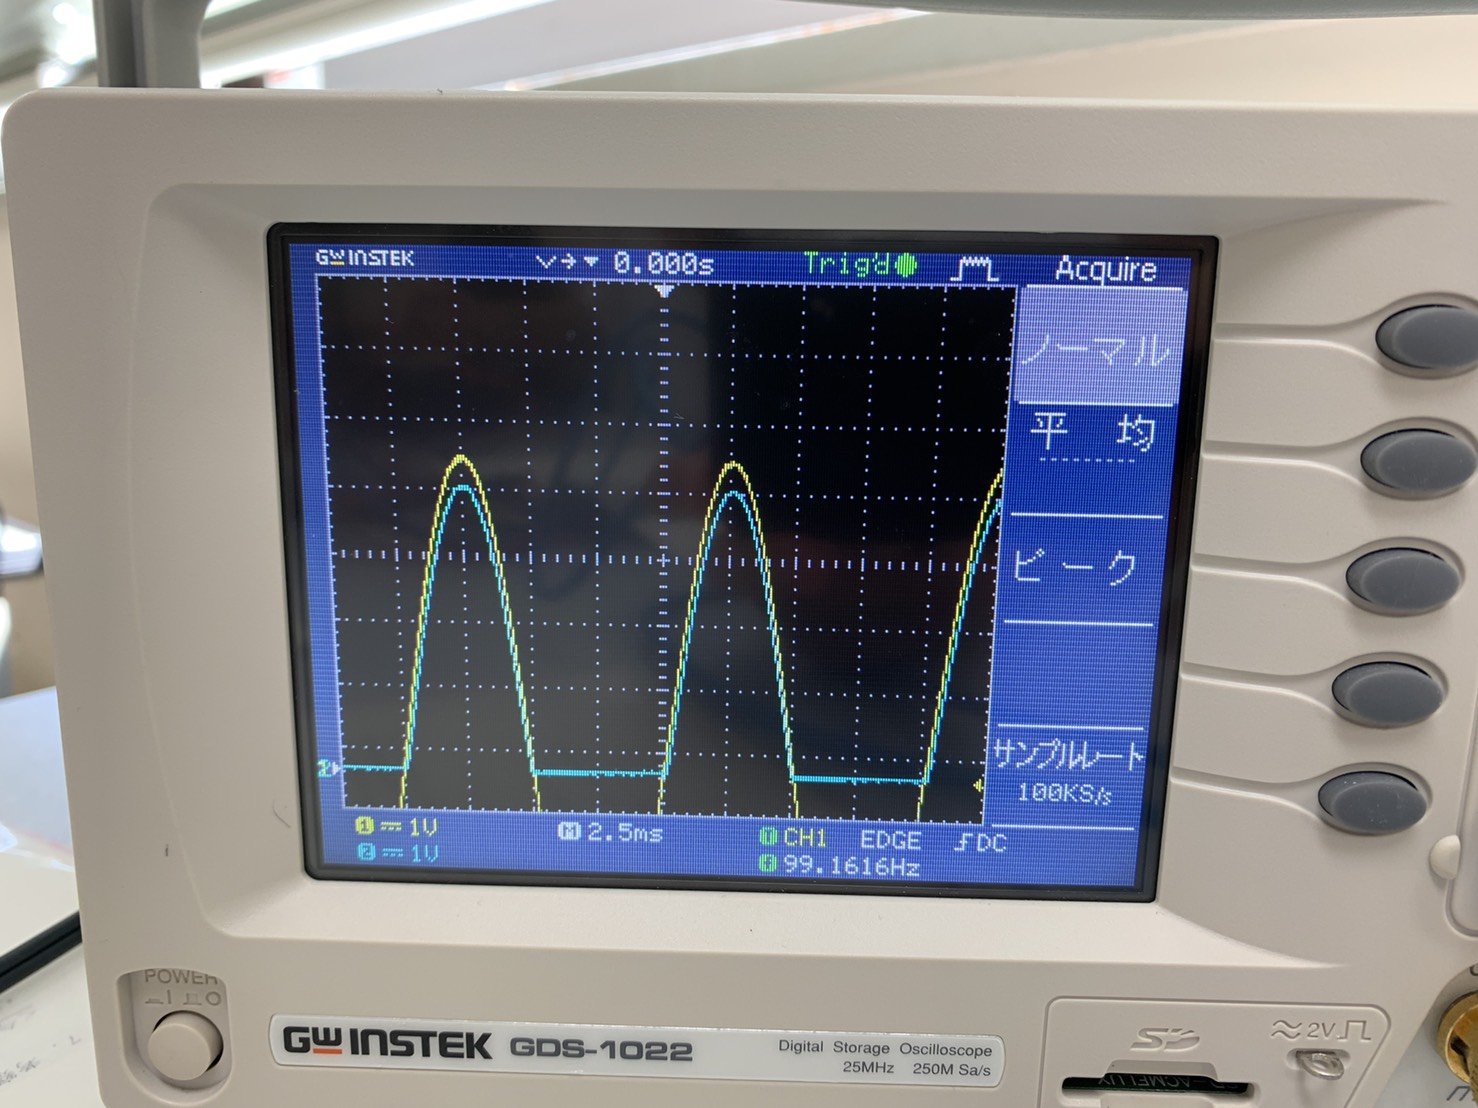
\includegraphics[width=10cm]{image/diode/S__19873810.jpg}
        \caption{半波整流回路測定の様子(1)}
        \label{fig:半波整流回路測定の様子(1)}
    \end{center}
\end{figure}

\begin{figure}[H]
    \begin{center}
        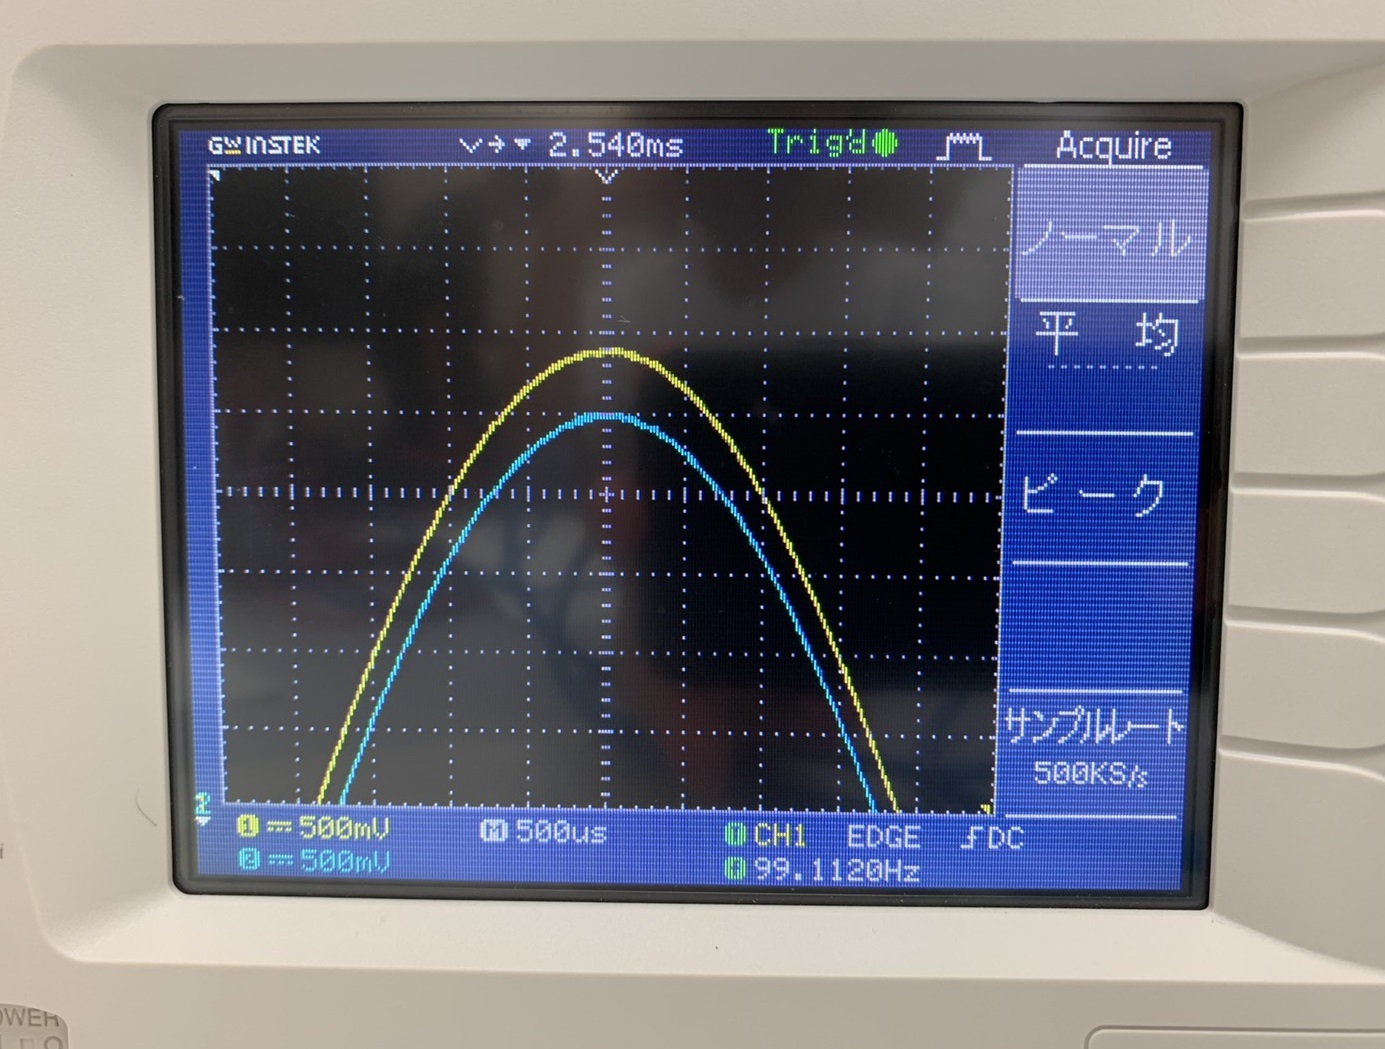
\includegraphics[width=10cm]{image/diode/S__19873806.jpg}
        \caption{半波整流回路測定の様子(2)}
        \label{fig:半波整流回路測定の様子(2)}
    \end{center}
\end{figure}

\begin{figure}[H]
    \begin{center}
        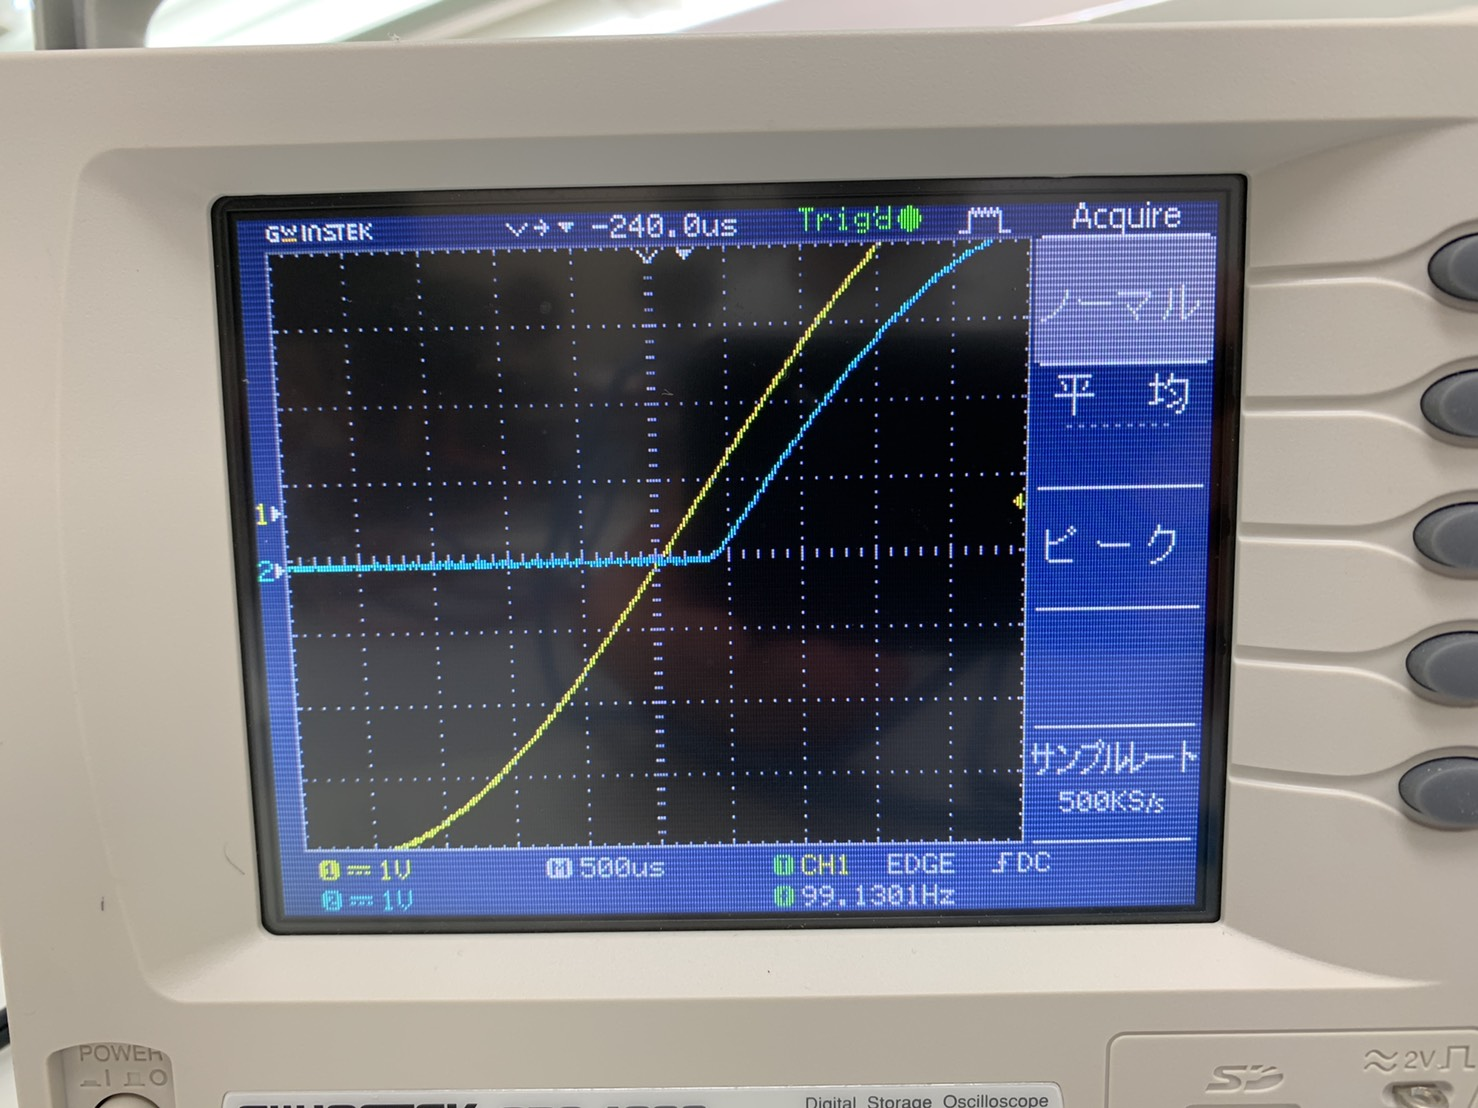
\includegraphics[width=10cm]{image/diode/S__19873811.jpg}
        \caption{半波整流回路測定の様子(3)}
        \label{fig:半波整流回路測定の様子(3)}
    \end{center}
\end{figure}

\begin{figure}[H]
    \begin{center}
        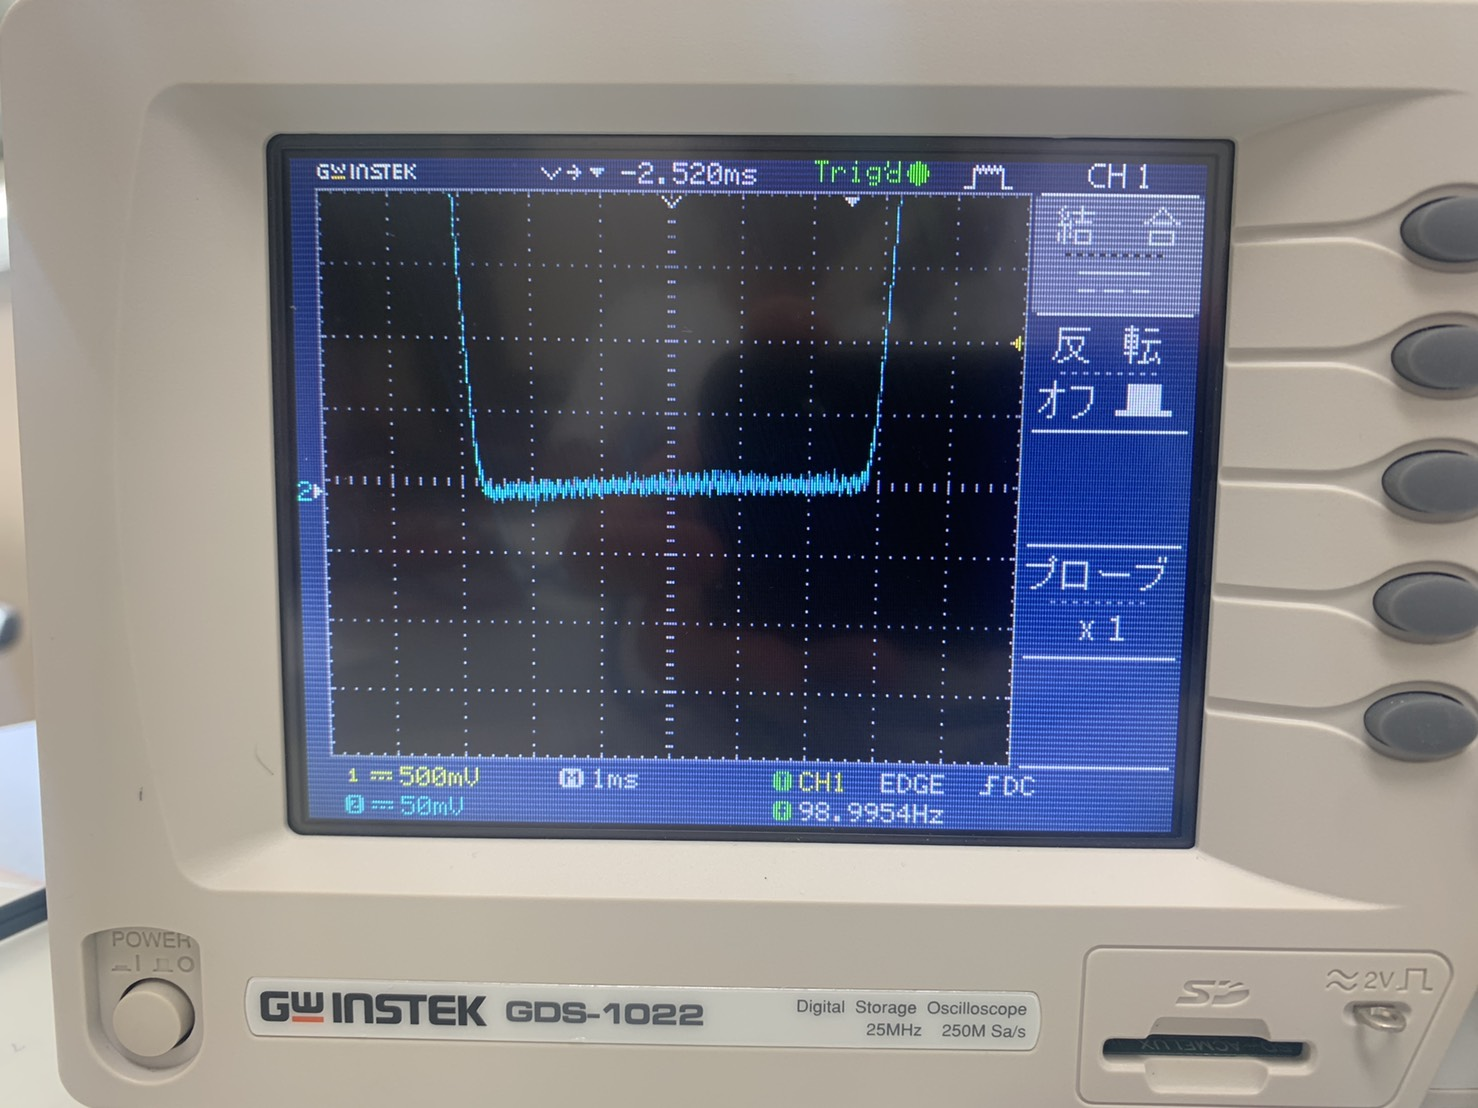
\includegraphics[width=10cm]{image/diode/S__19873802.jpg}
        \caption{半波整流回路測定の様子(4)}
        \label{fig:半波整流回路測定の様子(4)}
    \end{center}
\end{figure}

\begin{figure}[H]
    \begin{center}
        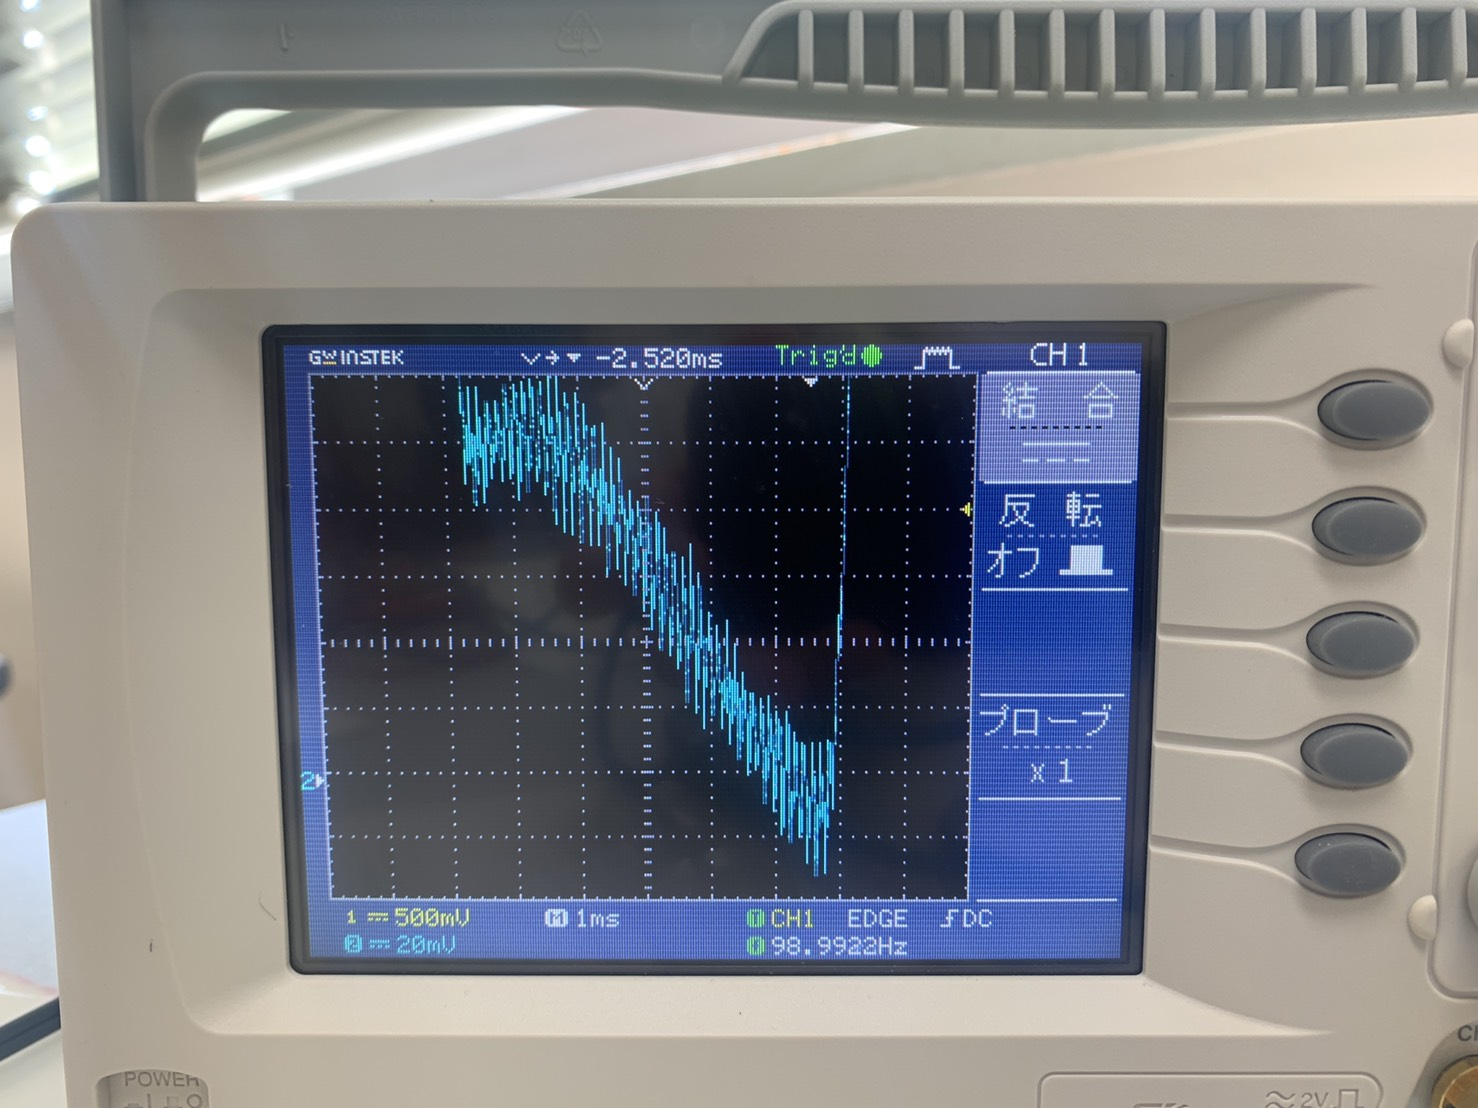
\includegraphics[width=10cm]{image/diode/S__19873801.jpg}
        \caption{半波整流回路測定の様子(5)}
        \label{fig:半波整流回路測定の様子(5)}
    \end{center}
\end{figure}


\subsection{考察}
\begin{figure}[H]
    \begin{center}
        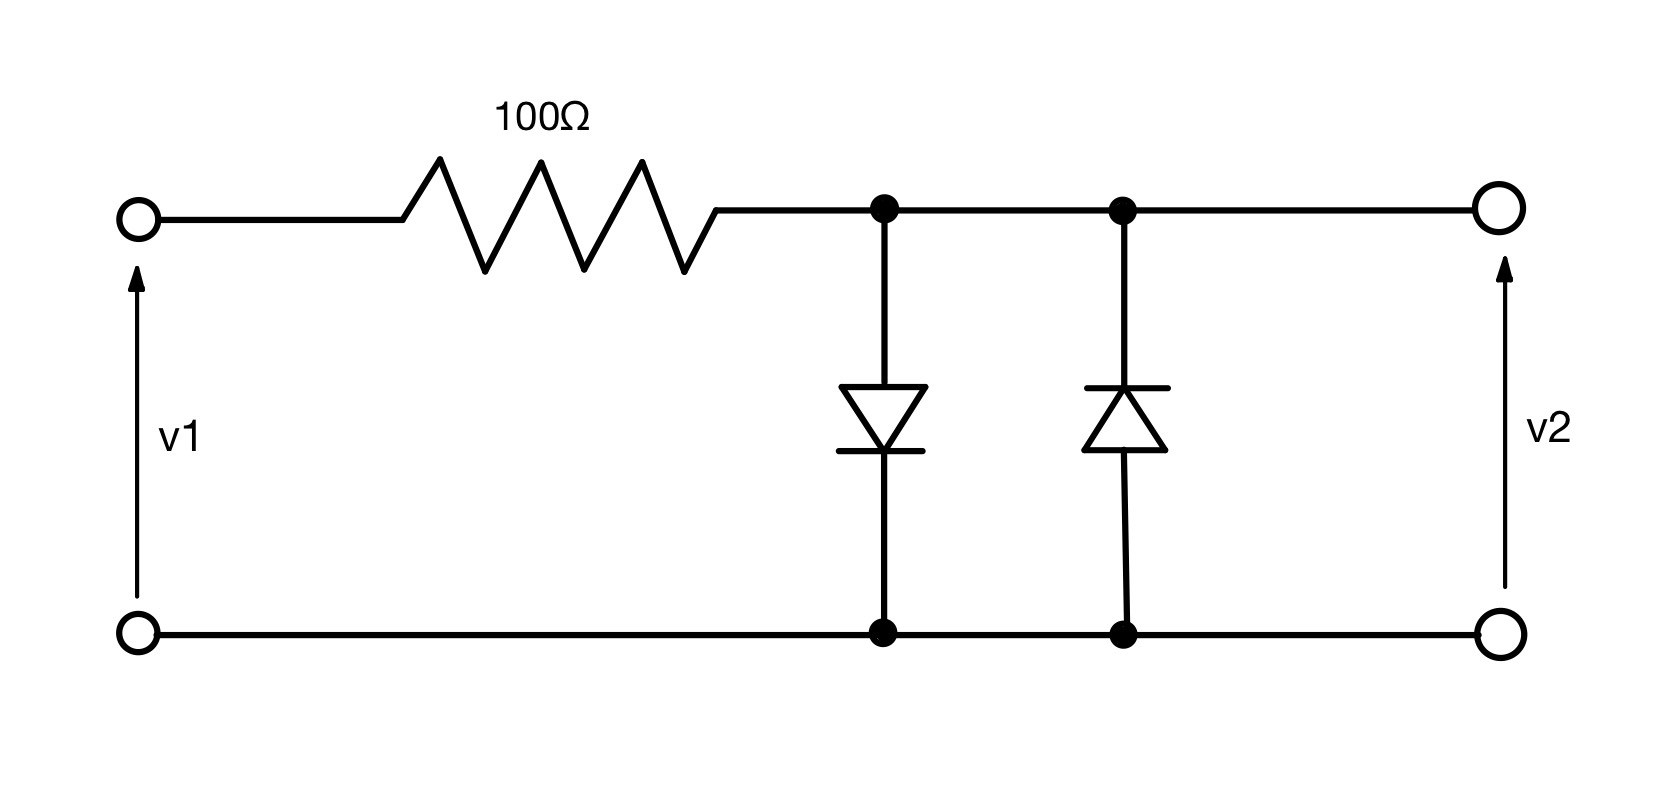
\includegraphics[width=10cm]{image/limmit.jpg}
        \caption{リミッタ}
        \label{fig:リミッタ}
    \end{center}
\end{figure}


\newpage
\section{実験B トランジスタの静特性}
\subsection{目的}
\begin{itemize}
    \item npn形トランジスタの静特性を測定し,その特性を把握する
    \item エミッタの設置回路について理解する
\end{itemize}
\subsection{使用器具}
\begin{enumerate}
    \item トランジスタ静特性評価回路 EC-07
    \item 直流安定化電源装置 KIKUSUI PMC35-2 L 48-10-1-42
    \item 直流安定化電源装置 TAKASAGO GPO25-5 帳1 番号195 分類B21
    \item デジタルマルチメータ SANWA CD770 EC-26, EC-35
    \item オシロスコープ GWINSTEK GDS-1022 No.2
\end{enumerate}

\subsection{トランジスタの原理}
\begin{figure}[H]
    \begin{center}
        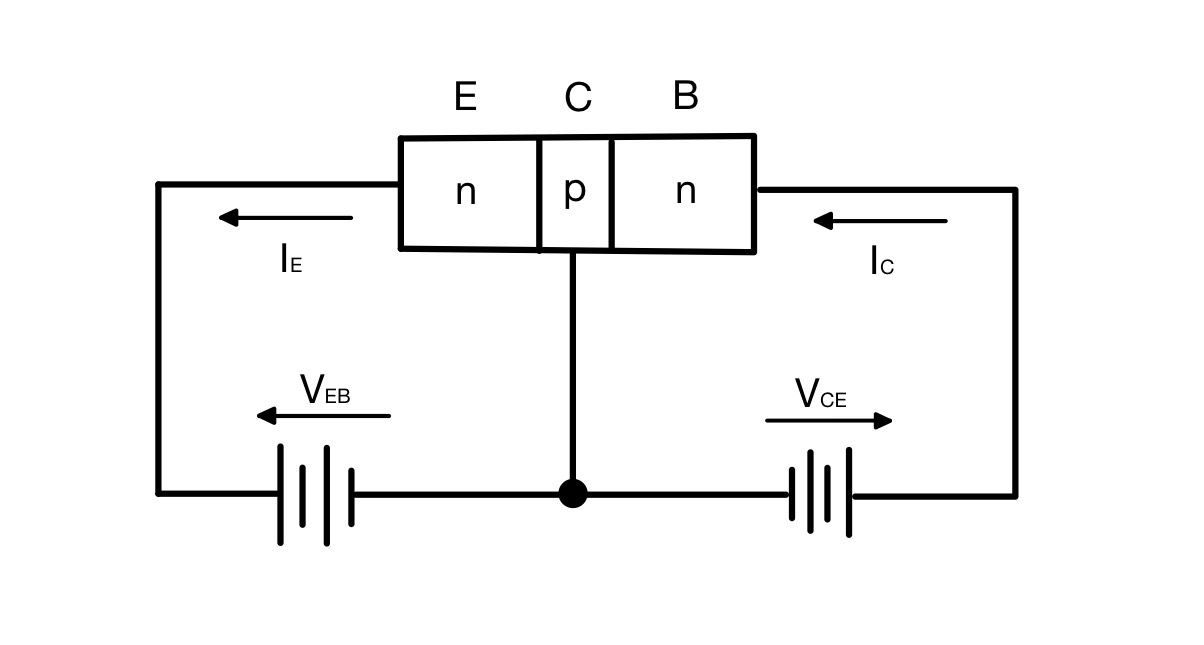
\includegraphics[width=10cm]{image/tr.jpg}
        \caption{ベース接地回路}
        \label{fig:ベース接地回路}
    \end{center}
\end{figure}

\subsection{評価回路の構造}
\begin{figure}[H]
    \begin{center}
        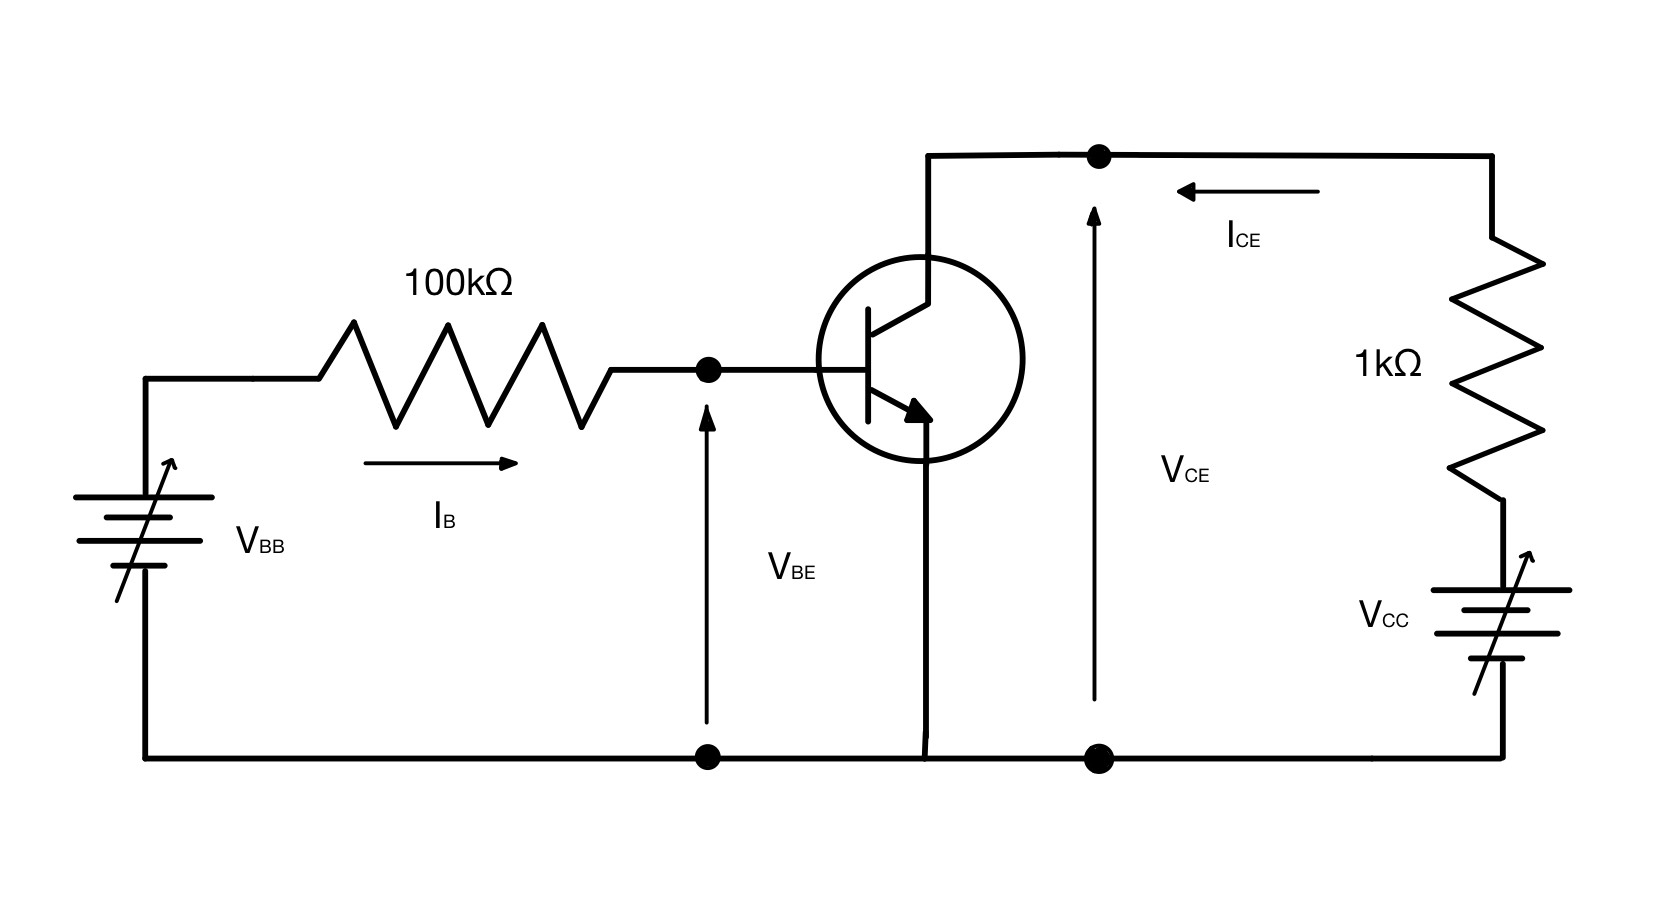
\includegraphics[width=10cm]{image/emitter.jpg}
        \caption{エミッタ接地回路}
        \label{fig:エミッタ接地回路}
    \end{center}
\end{figure}

\subsection{$V_{BE}$-$I_B$特性の測定}

\begin{table}[htbp]
    \caption{トランジスタ入力特性測定結果(0.5V)}
    \begin{center}
        \begin{tabular}{r|r|r|r|r|r}
            \hline\hline
            \multicolumn{1}{l|}{IB抵抗両端電圧[V]} & \multicolumn{1}{l|}{Vce[V]} & \multicolumn{1}{l|}{Ib[mA]} & \multicolumn{1}{l|}{IC抵抗両端電圧[V]} & \multicolumn{1}{l|}{Vbe[V]} & \multicolumn{1}{l}{Ic[mA]} \\ \hline
            1.398                                  & 0.502                       & 0.01398                     & 2.821                                  & 0.679                       & 0.002821                   \\ \hline
            0.671                                  & 0.496                       & 0.00671                     & 1.352                                  & 0.660                       & 0.001352                   \\ \hline
            0.392                                  & 0.500                       & 0.00392                     & 0.788                                  & 0.646                       & 0.000788                   \\ \hline
            0.371                                  & 0.500                       & 0.00371                     & 0.745                                  & 0.645                       & 0.000745                   \\ \hline
            0.289                                  & 0.500                       & 0.00289                     & 0.578                                  & 0.637                       & 0.000578                   \\ \hline
            0.138                                  & 0.498                       & 0.00138                     & 0.272                                  & 0.617                       & 0.000272                   \\ \hline
            0.060                                  & 0.499                       & 0.0006                      & 0.113                                  & 0.592                       & 0.000113                   \\ \hline
            0.022                                  & 0.498                       & 0.00022                     & 0.038                                  & 0.563                       & 3.8E-05                    \\ \hline
            0.001                                  & 0.500                       & 1E-05                       & 0.002                                  & 0.49                        & 2E-06                      \\ \hline
            0.000                                  & 0.502                       & 0                           & 0.000                                  & 0.034                       & 0                          \\ \hline
        \end{tabular}
    \end{center}
    \label{トランジスタ入力特性測定結果(0.5V)}
\end{table}

\begin{table}[htbp]
    \caption{トランジスタ入力特性測定結果(1.5V)}
    \begin{center}
        \begin{tabular}{r|r|r|r|r|r}
            \hline\hline
            \multicolumn{1}{l|}{IB抵抗両端電圧[V]} & \multicolumn{1}{l|}{Vce[V]} & \multicolumn{1}{l|}{Ib[mA]} & \multicolumn{1}{l|}{IC抵抗両端電圧[V]} & \multicolumn{1}{l|}{Vbe[V]} & \multicolumn{1}{l}{Ic[mA]} \\ \hline
            1.426                                  & 1.499                       & 0.01426                     & 2.913                                  & 0.678                       & 0.002913                   \\ \hline
            0.928                                  & 1.501                       & 0.00928                     & 1.899                                  & 0.666                       & 0.001899                   \\ \hline
            0.644                                  & 1.500                       & 0.00644                     & 1.318                                  & 0.657                       & 0.001318                   \\ \hline
            0.371                                  & 1.500                       & 0.00371                     & 0.755                                  & 0.642                       & 0.000755                   \\ \hline
            0.163                                  & 1.499                       & 0.00163                     & 0.326                                  & 0.62                        & 0.000326                   \\ \hline
            0.062                                  & 1.503                       & 0.00062                     & 0.118                                  & 0.591                       & 0.000118                   \\ \hline
            0.011                                  & 1.499                       & 0.00011                     & 0.016                                  & 0.538                       & 1.6E-05                    \\ \hline
            0.002                                  & 1.502                       & 1.9E-05                     & 0.003                                  & 0.495                       & 3E-06                      \\ \hline
            0.000                                  & 1.503                       & 0                           & 0.000                                  & 0.034                       & 0                          \\ \hline
        \end{tabular}
    \end{center}
    \label{トランジスタ入力特性測定結果(1.5V)}
\end{table}

\begin{table}[htbp]
    \caption{トランジスタ入力特性測定結果(2.5V)}
    \begin{center}
        \begin{tabular}{r|r|r|r|r|r}
            \hline
            \multicolumn{1}{l|}{IB抵抗両端電圧[V]} & \multicolumn{1}{l|}{Vce[V]} & \multicolumn{1}{l|}{Ib[mA]} & \multicolumn{1}{l|}{IC抵抗両端電圧[V]} & \multicolumn{1}{l|}{Vbe[V]} & \multicolumn{1}{l}{Ic[mA]} \\ \hline
            1.403                                  & 2.505                       & 0.01403                     & 2.883                                  & 0.677                       & 0.002883                   \\ \hline
            0.957                                  & 2.503                       & 0.00957                     & 1.995                                  & 0.667                       & 0.001995                   \\ \hline
            0.352                                  & 2.500                       & 0.00352                     & 0.728                                  & 0.642                       & 0.000728                   \\ \hline
            0.193                                  & 2.498                       & 0.00193                     & 0.386                                  & 0.626                       & 0.000386                   \\ \hline
            0.109                                  & 2.503                       & 0.00109                     & 0.215                                  & 0.612                       & 0.000215                   \\ \hline
            0.021                                  & 2.497                       & 0.00021                     & 0.049                                  & 0.566                       & 4.9E-05                    \\ \hline
            0.007                                  & 2.499                       & 7E-05                       & 0.011                                  & 0.534                       & 1.1E-05                    \\ \hline
            0.000                                  & 2.503                       & 0                           & 0.000                                  & 0.034                       & 0                          \\ \hline
        \end{tabular}
    \end{center}
    \label{トランジスタ入力特性測定結果(2.5V)}
\end{table}


\begin{figure}[H]
    \begin{center}
        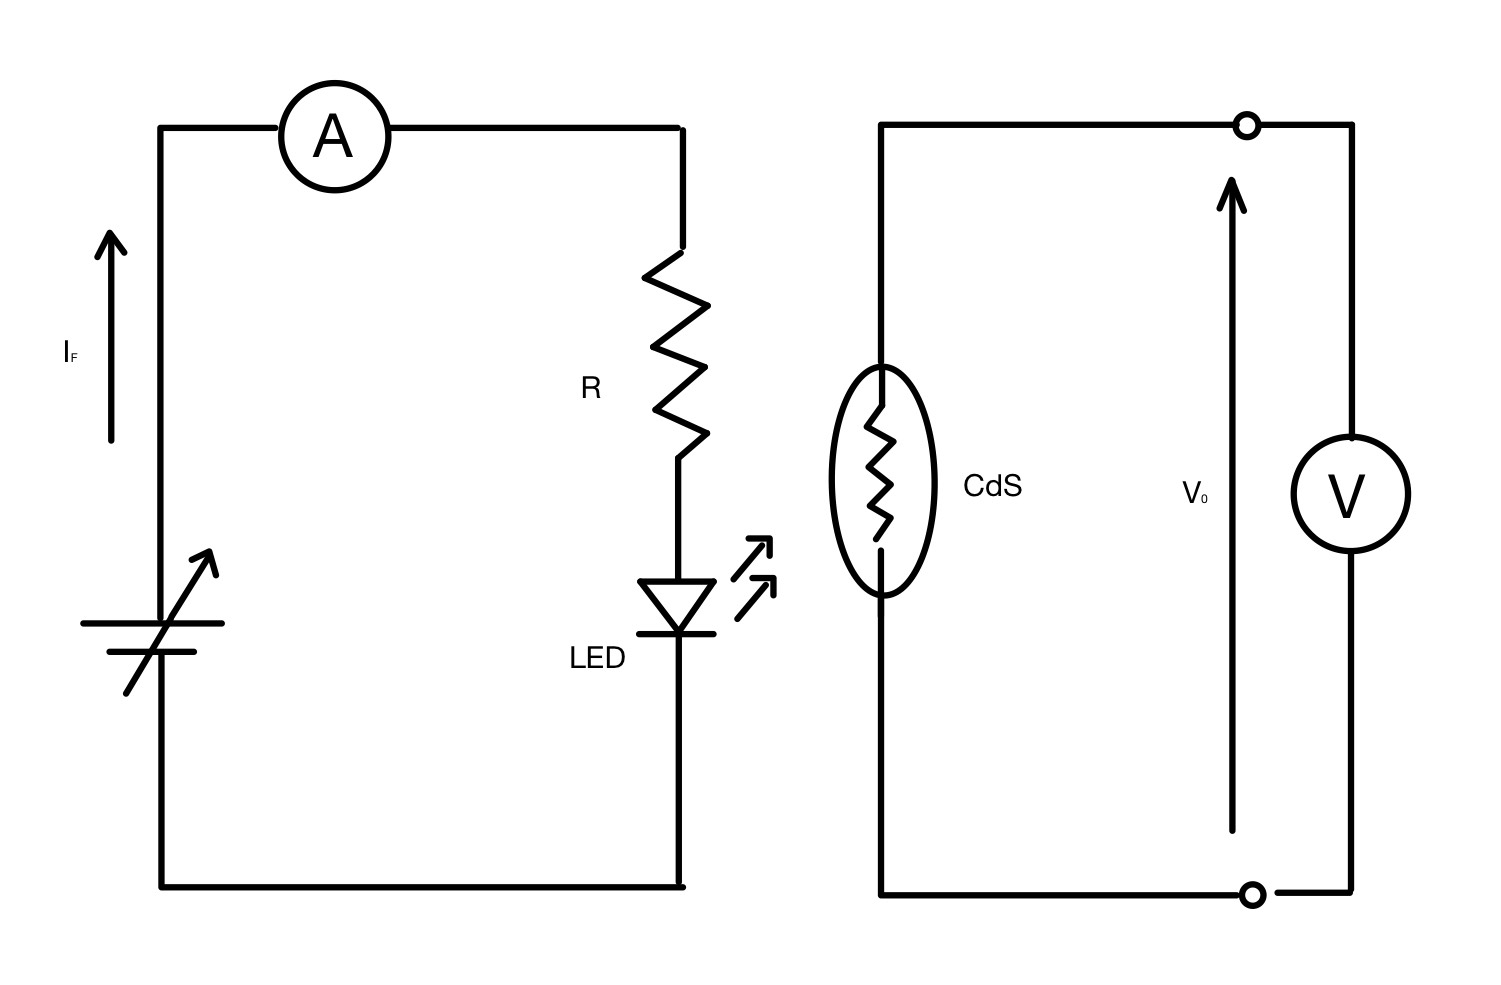
\includegraphics[width=10cm]{graph/5.png}
        \caption{トランジスタ入力特性測定結果(グラフ)}
        \label{fig:トランジスタ入力特性測定結果(グラフ)}
    \end{center}
\end{figure}

\subsection{$V_{CE}$-$I_C$特性の測定}

\begin{table}[htbp]
    \caption{トランジスタ出力特性測定結果(2μA)}
    \begin{center}
        \begin{tabular}{r|r|r}
            \hline\hline
            \multicolumn{1}{l|}{Vce[V]} & \multicolumn{1}{l|}{IC抵抗両端電圧[V]} & \multicolumn{1}{l}{Ic[mA]} \\ \hline
            9.980                       & 0.413                                  & 0.413                      \\ \hline
            6.070                       & 0.409                                  & 0.409                      \\ \hline
            5.000                       & 0.409                                  & 0.409                      \\ \hline
            3.004                       & 0.403                                  & 0.403                      \\ \hline
            1.502                       & 0.404                                  & 0.404                      \\ \hline
            1.004                       & 0.404                                  & 0.404                      \\ \hline
            0.507                       & 0.400                                  & 0.400                      \\ \hline
            0.245                       & 0.388                                  & 0.388                      \\ \hline
            0.195                       & 0.363                                  & 0.363                      \\ \hline
            0.151                       & 0.295                                  & 0.295                      \\ \hline
            0.101                       & 0.117                                  & 0.117                      \\ \hline
            0.049                       & 0.016                                  & 0.016                      \\ \hline
            0.000                       & 0.001                                  & 0.001                      \\ \hline
        \end{tabular}
    \end{center}
    \label{トランジスタ出力特性測定結果(2μA)}
\end{table}

\begin{table}[htbp]
    \caption{トランジスタ出力特性測定結果(4μA)}
    \begin{center}
        \begin{tabular}{r|r|r}
            \hline\hline
            \multicolumn{1}{l|}{Vce[V]} & \multicolumn{1}{l|}{IC抵抗両端電圧[V]} & \multicolumn{1}{l}{Ic[mA]} \\ \hline
            9.950                       & 0.845                                  & 0.845                      \\ \hline
            6.110                       & 0.835                                  & 0.835                      \\ \hline
            3.055                       & 0.825                                  & 0.825                      \\ \hline
            1.511                       & 0.820                                  & 0.820                      \\ \hline
            1.081                       & 0.818                                  & 0.818                      \\ \hline
            0.513                       & 0.814                                  & 0.814                      \\ \hline
            0.253                       & 0.792                                  & 0.792                      \\ \hline
            0.149                       & 0.545                                  & 0.545                      \\ \hline
            0.105                       & 0.265                                  & 0.265                      \\ \hline
            0.000                       & 0.000                                  & 0.000                      \\ \hline
        \end{tabular}
    \end{center}
    \label{トランジスタ出力特性測定結果(4μA)}
\end{table}

\begin{table}[htbp]
    \caption{トランジスタ出力特性測定結果(6μA)}
    \begin{center}
        \begin{tabular}{r|r|r}
            \hline\hline
            \multicolumn{1}{l|}{Vce[V]} & \multicolumn{1}{l|}{IC抵抗両端電圧[V]} & \multicolumn{1}{l}{Ic[mA]} \\ \hline
            9.970                       & 1.250                                  & 1.250                      \\ \hline
            1.009                       & 1.230                                  & 1.230                      \\ \hline
            0.490                       & 1.220                                  & 1.220                      \\ \hline
            0.245                       & 1.190                                  & 1.190                      \\ \hline
            0.204                       & 1.140                                  & 1.140                      \\ \hline
            0.152                       & 0.904                                  & 0.904                      \\ \hline
            0.103                       & 0.377                                  & 0.377                      \\ \hline
            0.052                       & 0.062                                  & 0.062                      \\ \hline
            0.000                       & 0.001                                  & 0.001                      \\ \hline
        \end{tabular}
    \end{center}
    \label{トランジスタ出力特性測定結果(6μA)}
\end{table}

\begin{table}[htbp]
    \caption{トランジスタ出力特性測定結果(8μA)}
    \begin{center}
        \begin{tabular}{r|r|r}
            \hline
            \multicolumn{1}{l|}{Vce[V]} & \multicolumn{1}{l|}{IC抵抗両端電圧[V]} & \multicolumn{1}{l}{Ic[mA]} \\ \hline
            9.980                       & 1.670                                  & 1.670                      \\ \hline
            1.040                       & 1.618                                  & 1.618                      \\ \hline
            0.517                       & 1.606                                  & 1.606                      \\ \hline
            0.254                       & 1.572                                  & 1.572                      \\ \hline
            0.197                       & 1.486                                  & 1.486                      \\ \hline
            0.151                       & 1.180                                  & 1.180                      \\ \hline
            0.106                       & 0.500                                  & 0.500                      \\ \hline
            0.048                       & 0.070                                  & 0.070                      \\ \hline
            0.009                       & -0.013                                 & -0.013                     \\ \hline
        \end{tabular}
    \end{center}
    \label{トランジスタ出力特性測定結果(8μA)}
\end{table}

\begin{table}[htbp]
    \caption{トランジスタ出力特性測定結果(10μA)}
    \begin{center}
        \begin{tabular}{r|r|r}
            \hline
            \multicolumn{1}{l|}{Vce[V]} & \multicolumn{1}{l|}{IC抵抗両端電圧[V]} & \multicolumn{1}{l}{Ic[mA]} \\ \hline
            9.970                       & 2.119                                  & 2.119                      \\ \hline
            1.063                       & 2.048                                  & 2.048                      \\ \hline
            0.479                       & 2.030                                  & 2.030                      \\ \hline
            0.256                       & 2.000                                  & 2.000                      \\ \hline
            0.197                       & 1.893                                  & 1.893                      \\ \hline
            0.150                       & 1.468                                  & 1.468                      \\ \hline
            0.098                       & 0.553                                  & 0.553                      \\ \hline
            0.004                       & -0.006                                 & -0.006                     \\ \hline
        \end{tabular}
    \end{center}
    \label{トランジスタ出力特性測定結果(10μA)}
\end{table}


\begin{figure}[H]
    \begin{center}
        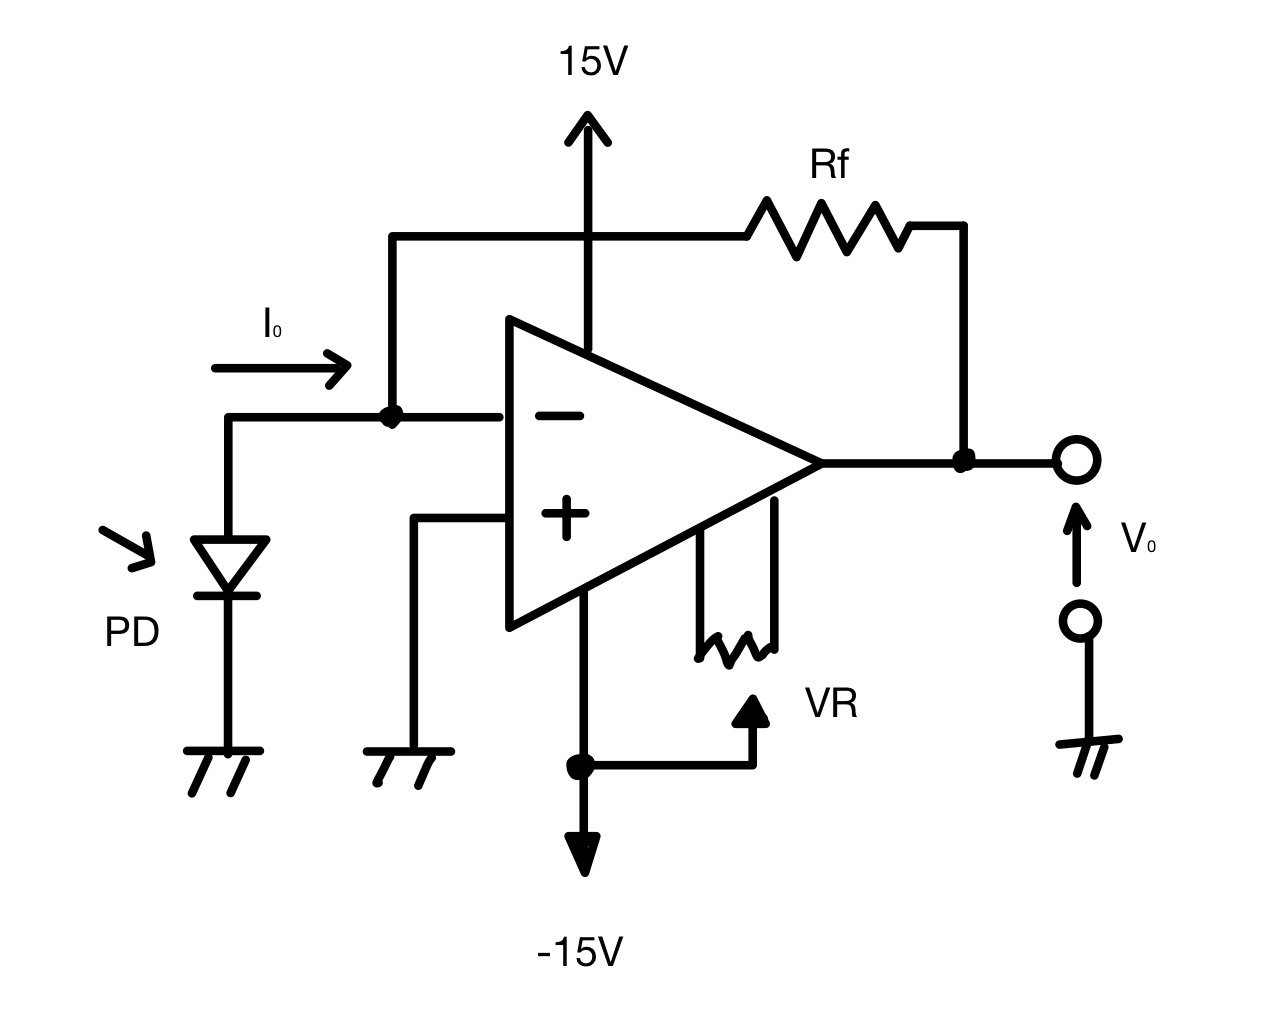
\includegraphics[width=10cm]{graph/6.png}
        \caption{トランジスタ出力特性測定結果(グラフ)}
        \label{fig:トランジスタ出力特性測定結果(グラフ)}
    \end{center}
\end{figure}

\begin{figure}[H]
    \begin{center}
        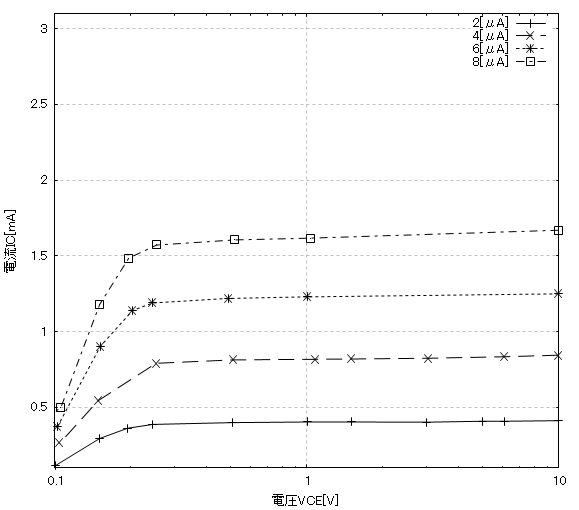
\includegraphics[width=10cm]{graph/6t.png}
        \caption{トランジスタ出力特性測定結果(対数グラフ)}
        \label{fig:トランジスタ出力特性測定結果(対数グラフ)}
    \end{center}
\end{figure}
\subsection{考察}

\newpage
\section{感想}

\begin{thebibliography}{99}
    \bibitem{}皆川正寛,「半導体素子の静特性の測定,令和3年度電子制御工学実験・3年前期テキスト」
    %\bibitem{竹部}竹部啓輔, 「{\TeX}によるレポート作成,令和3年度電子制御工学実験・3年前期テキスト pp.A-1-A-18, (2021/4.
\end{thebibliography}

\end{document}